%!TEX root = ../../../super_main.tex

\section{Inconsistent Tab Size in Settings Panel}
\label{sec:inconsistent_tab_size_in_settings_panel}

In the settings view of the \launcher application, the user is presented with different tabs containing settings for \emph{some} of the different parts of the overall \giraf-application. Each of these tabs contains a headline and a small description of the tab. However, when a setting pane is pressed, the description disappears. This causes the size of the tab to change, which can be confusing for the users. An example of the problem can be seen on \figref{fig:inconsistent_tab_size_in_settings_panel_example}.

\begin{figure}[!htbp]
    \centering

    \begin{subfigure}[t]{0.3\textwidth}
        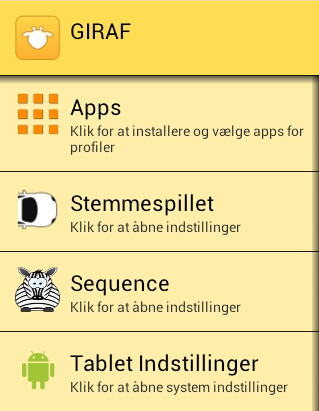
\includegraphics[width=\textwidth]{sprint_one/inconsistent_tab_size_in_settings_panel/example_one}
        \caption{\emph{GIRAF}-tab selected}
        \label{fig:inconsistent_tab_size_in_settings_panel_example_one}
    \end{subfigure}
    \hspace{5em} 
    \begin{subfigure}[t]{0.3\textwidth}
        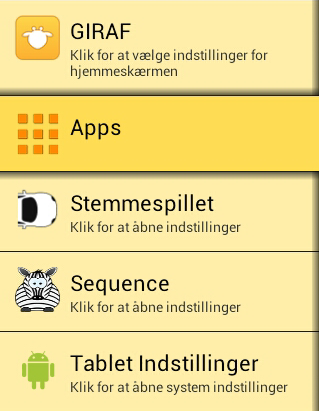
\includegraphics[width=\textwidth]{sprint_one/inconsistent_tab_size_in_settings_panel/example_two}
        \caption{\emph{Apps}-tab selected}
        \label{fig:inconsistent_tab_size_in_settings_panel_example_two}
    \end{subfigure}
    
    \caption{Problem visualized}
    \label{fig:inconsistent_tab_size_in_settings_panel_example}
\end{figure}

A way to solve the problem would be to always show the description, however this does not make much sense because the description is used to indicate what the user might expect to find under the different tabs. For instance the description for the \emph{GIRAF}-tab reads \translated{Klik for at vælge indstillinger for hjemmeskærmen}{Click to choose settings for the home screen}. This text does not make much sense to show when the \emph{GIRAF}-tab is already selected because of two reasons, namely that a click cannot be made since the tab is already active. Besides this, the content corresponding to the settings-tab is shown to the user, so the user could just look at what settings are available and should not need any further instructions to what is available.
\\\\
Another idea would be to remove the descriptions and make the headlines more descriptive. This is a good approach since the only motivation for the existence of the descriptions is the somewhat vague headlines. Let us for instance consider the \emph{GIRAF}-headline. This headline needs a description since it is very unclear what the user might find under this tab. However, if the tab were to be renamed to \translated{Generelt}{General} the user will have a much better understanding of the content of this tab. Besides this, let us consider the tabs \emph{Stemmespillet} and \emph{Sequence}. These two tabs share the same description \translated{Klik for at åbne indstillinger}{Click to open settings}. This description is very basic and vague and thus not needed. Besides this, the user should already be aware that the different tabs will open different setting panes.

\subsection{Solution}
\label{sub:inconsistent_tab_size_in_settings_panel_solution}
\figref{fig:inconsistent_tab_size_in_settings_panel_example_solution} shows the implemented solution. It is clear to see that the tab size is consistent and no unclear description texts are shows. Besides this, both the text and the icon has been vertically aligned accordingly to the tab. The first tab has been relabeled to \translated{Generelt}{General}, while the second tab has been relabeled to \translated{Aktive applikationer}{Active applications}.

\begin{figure}[!htbp]
    \centering

    \begin{subfigure}[t]{0.3\textwidth}
        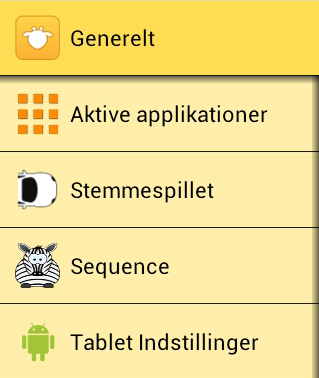
\includegraphics[width=\textwidth]{sprint_one/inconsistent_tab_size_in_settings_panel/example_three}
        \caption{\emph{Generel}-tab selected}
        \label{fig:inconsistent_tab_size_in_settings_panel_example_one_solution}
    \end{subfigure}
    \hspace{5em} 
    \begin{subfigure}[t]{0.3\textwidth}
        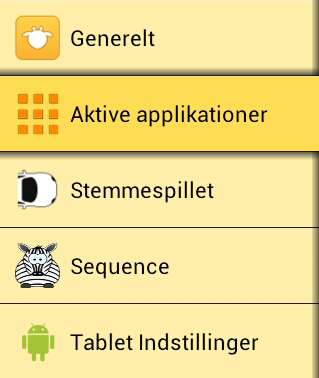
\includegraphics[width=\textwidth]{sprint_one/inconsistent_tab_size_in_settings_panel/example_four}
        \caption{\emph{Aktive applikationer}-tab selected}
        \label{fig:inconsistent_tab_size_in_settings_panel_example_two_solution}
    \end{subfigure}
    
    \caption{Solution visualized}
    \label{fig:inconsistent_tab_size_in_settings_panel_example_solution}
\end{figure}